\documentclass[a4paper, 11pt]{article}
\usepackage[a4paper, left=2.25cm, right=2.25cm, top=2cm, bottom=2cm]{geometry}
\usepackage{multirow}
\usepackage{arydshln}
\usepackage{epstopdf}
\usepackage{graphicx}
\usepackage{booktabs}
%\usepackage[style=authoryear]{biblatex}
%\usepackage{natbib}
\usepackage[numbers]{natbib}
\usepackage{chngcntr}
\usepackage{epsfig}
\usepackage{float}
\usepackage{listings}
\lstset{
	basicstyle=\ttfamily,
	columns=flexible,
	breaklines=true
}
\usepackage[dvipsnames]{color}
\usepackage{subfigure}
\usepackage{verbatim}
\usepackage{enumerate}
\usepackage{soul}
\usepackage{url}
\usepackage{amsmath}
\usepackage{amssymb}
\makeatletter
\newcommand{\figcaption}{\def\@captype{figure}\caption}
\newcommand{\tabcaption}{\def\@captype{table}\caption}
\makeatother

\title{\bf SBic: A comprehensive pipeline that implements\\
  sequential biclustering for immune evasion subtype\\
  identification and follow-up analysis of cancer patients}
\author{Yuhang Liu, Mayassa J. Bou-Dargham,\\ 
  Qing-Xiang Amy Sang, and Jinfeng Zhang}

\begin{document}
\date{September 3, 2017}
\maketitle
\setlength{\parindent}{0pt}
\section*{0 Introduction}
\subsection*{0.1 Background}
Breast cancer (BRCA) may escape immune surveillance using $6$ known evasion mechanisms, yet it is not fully understood which mechanism or combination of mechanisms are used by subsets of human BRCA patients. Activation of multiple immune evasion mechanisms simultaneously in a single cancer may explain the ineffectiveness of an immunotherapy in certain patients targeting on a single mechanism. An illustration is also given in Figure~\ref{fig:immu-mech}. Characterization of the BRCA immune evasion subtypes (IES) is essential for a better understanding of patient responses to immunotherapies (especially the cases of ineffectiveness) and for rational clinical trial design of combination immunotherapies.

\subsection*{0.2 Results}
Using the RNA-seq data of BRCA from The Cancer Genome Atlas (TCGA), \textbf{seven} IES were identified for $81$\% of our study population. These IES utilize $7$ different combinations of the six evasion mechanisms (M1-M6): IES 1 (M1, M2, M3, M4); IES 2 (M5); IES 3 (M1, M4, M5); IES 4 (M6); IES 5 (M1, M5); IES 6 (M1, M2, M4, M5); and IES 7 (M1, M2), which represent $27.8$\%, $4.2$\%, $13.4$\%, $10.1$\%, $10.4$\%, $5.6$\% and $5.5$\% of the total patients, respectively. Approximately half of the triple negative breast cancer (TNBC) patients falls into subtype $1$ and another half subtype $2$. We also identified biomarkers that help classify a patient into one of the IES.

\subsection*{0.3 Conclusions}
This study unravels a complex picture of immune evasion mechanisms of BRCA. While implying a challenging path ahead for treating BRCA with immunotherapies, the identified IES and their corresponding biomarkers provide guidance for rational design of combination immunotherapies in clinical trials by optimizing the choice of treatments and patient selection. In terms of statistical procedures, sequential biclustering, differential expression $t$-tests, classification and (cross validated) prediction are involved. Going one step further, the goal of our package is to compile all these procedures into a pipeline and make it general for different types of cancer and whatever gene list of interest.
\begin{figure}[!tpb]
  \begin{center}
    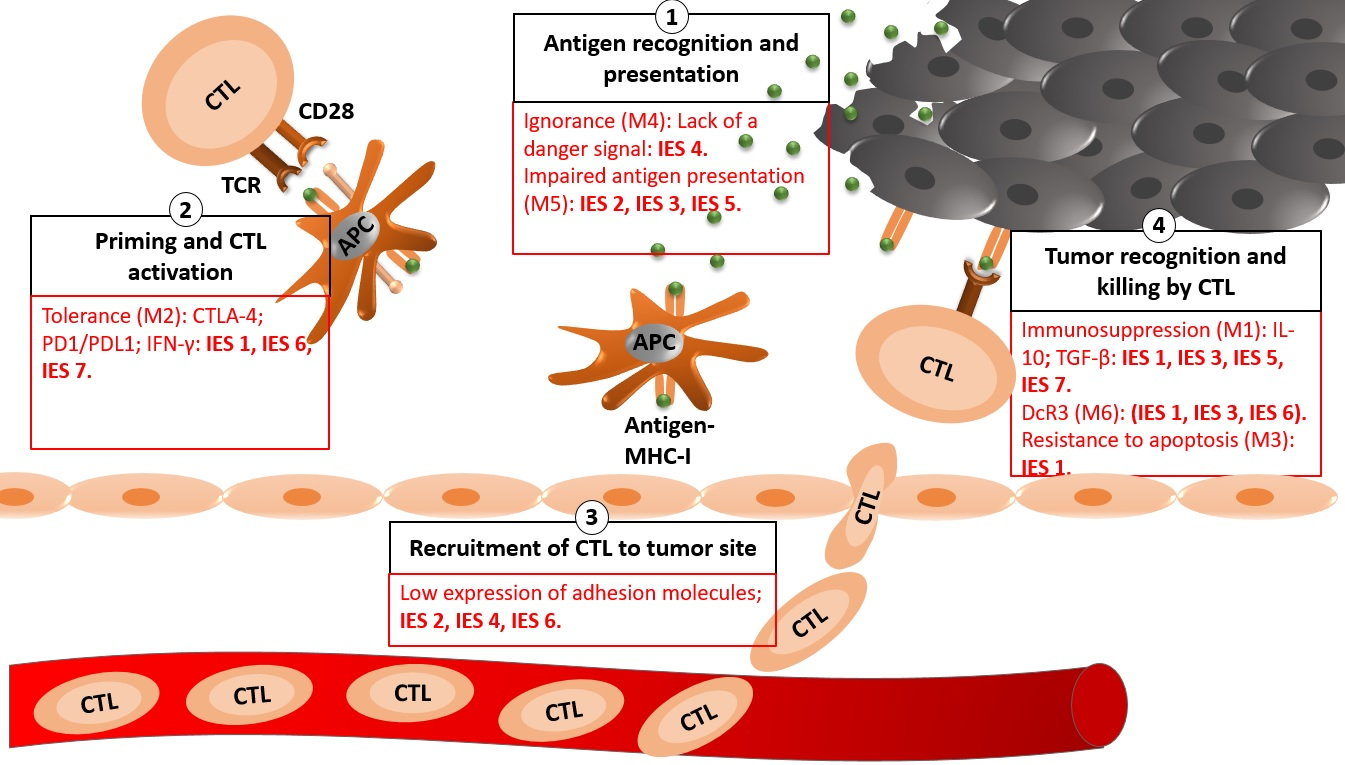
\includegraphics[width=12 cm]{Figure1-final.jpg}
    \caption{An illustration of immune evasion mechanism of cancer patients}
    \label{fig:immu-mech}
  \end{center}
\end{figure}

\section*{1 Materials and Methods}
\subsection*{1.1 Immune Related Gene List with Protein-protein Interaction}
Based on the knowledge of the mechanism of tumor evasion from immune system destruction, a list of $87$ genes was generated manually based on the available literature (Supplementary file 1 of our companion paper). The generated list included genes involved in the cancer-immunity cycle, and tolerance and immunosuppression-inducing genes. To make sure no important genes were missing, the list was expanded from $87$ to $1,356$ genes through adding all interacting proteins determined using bioGRID database (\url{https://thebiogrid.org/}). The data are publicly available from The Cancer Genomic Atlas (TCGA).

\subsection*{1.2 Sequential Biclustering}
Biclustering, also known as block clustering, co-clustering, or two-way clustering, is the technique of simultaneously clustering the rows and columns of a matrix. In our study, biclustering shuffles rows (genes) and columns (patients) of the data matrix to generate clusters with minimum variation of gene expression amongst a group of patients (intra-cluster variation) and maximum variation with other groups of patients (inter-cluster variation). We used the \texttt{biclust} package available in R on the Log2-transformed gene expression data of cancer patients to divide patients into subgroups based on their expression of immune genes. The BCPlaid algorithm~\citep{turner2005improved, lazzeroni2002plaid} was used as it clusters patients (columns) based on their similarity in gene expression (row-based) rather than by similar gene expression per patient (column-based). Running the BCPlaid generated overlapping clusters of patients and genes, where the clusters are ranked based on their degree of coherence of genes. Since our goal is to divide patients into groups, where one patient should fall in only one group, we adopted a sequential approach. In this procedure, we run the BCPlaid algorithm multiple times \textit{sequentially}. After each run, we take the top-ranked cluster with at least $5$\% of the cancer patients and remove the patients in this cluster from the set of patients who are being clustered. The remaining patients will be clustered in the next run. The constraint of each candidate cluster having at least $5$\% of the cancer patients guarantees that finally, each immune evasion subtype (IES) is a representative set of patients from the study population.
\begin{lstlisting}
SBic <- function(X, propcutoff = 0.05, seed = 1234, outopt = "table", 
				Dataname = "Dataset") {
	...
}
\end{lstlisting}
\begin{itemize}
\item \texttt{X} is the input expression matrix, where we follow the convention that genes are on rows and samples are on columns.
\item \texttt{propcutoff} is the \textit{minimum} proportion of samples for a valid sequential bicluster. For example, if total number of samples is $1,000$ and \texttt{propcutoff}$=0.05$, then each output bicluster must at least have $50$ samples.
\item \texttt{seed} is the random number seed for running biclustering. It is set back to the same number after each iteration is finished.
\item \texttt{outopt} is the output option. Default is ``\texttt{table}", which means that the program will automatically output sequential biclusters in matrix format as text file tables.
\item \texttt{Dataname} is an appropriate prefix of the output file names. For example, if the data is breast cancer RNA-seq, we can use \texttt{Datanametrt}=\texttt{BRCARNAseq}
\end{itemize}

\subsection*{1.3 A General Differential Expression Function}
We follow the convention that gene expressions are arranged in a matrix where each row represents a gene and each column represents a sample. We further assume that the input data of this function is after necessary normalization and on \textbf{log2} scale. For simplicity, we recommend pooling two groups into a single matrix $X$. The input \texttt{classlabel} is a vector of length equal to the number of columns of $X$. It can be either numeric, character, or factor, but it needs to have two unique values. The underlying procedure is a two-sided $t$-test. Test statistics and \textit{raw} $p$-values are returned for further investigation. If the matrix $X$ contains any missing value, the program will continue implementing the tests and print out notification which gene(s) have missing value(s).
\begin{verbatim}
ttest_general <- function (X, classlabel) 
{
  ...
}
\end{verbatim}
\begin{itemize}
\item \texttt{X} is the \textit{pooled} expression matrix with both clinical or phenotypic groups, where we follow the convention that genes are on rows and samples are on columns.
\item \texttt{classlabel} is a vector with the group labels. Its length must equal the number of columns of \texttt{X}. It can be either numeric, character, or factor, but it must have two unique values.
\end{itemize}

\subsection*{1.4 Pathway Analysis}
To find out whether an immune pathway is altered in each of the $7$ IES, we compared expression of genes in a IES with those of other IES (tumor) and normal samples. The significantly differentially expressed genes and the corresponding \textbf{KEGG} pathways were plotted using the R/Bioconductor package \texttt{pathview} for visualization~\citep{luo2013pathview}. We have chosen the immune related pathways and shown only the pathways for antigen processing and presentation (hsa04612), leukocyte transendothelial migration (hsa04670), and cell adhesion molecules (hsa04514) that also shows the fold change of PD-1 (PDCD1), PD-L2 (PDCD1LG2), and CTLA4.\\
$T$-tests were implemented to compare the mean expression of a gene within an IES to the mean expression of other cancer patients and to that of normal samples (Supplementary file 4). To analyze the $t$-test results, the genes were categorized into different groups based on their role in the cancer-immunity cycle (Supplementary file 4). Using the generated $p$-values for the tumor-tumor and tumor-normal mean expressions, we were able to understand at which level evasion was happening and using which molecules. We skip the computer program and output of this part because they may take unnecessarily large space, and may not affect the main part of the computational pipeline. \hl{Interested readers please refer to our companion paper or request from the author for more details.}

\subsection*{1.5 Heatmap Visualization of Cancer Data}
We also create a heatmap for better visualization of the $7$ IES. The expressions used for this heatmap are standardized by the per-gene mean and standard deviation. Patients are ordered from IES 1 (left) to IES 7 (right), identified by the color bars above the heatmap. \hl{The ordering strategy of genes (i.e. the file \textit{gene\_assignment.txt}) can be provided by the author upon request}. Considering the variety of ways to plot a heatmap in \texttt{R}, the code provided above is only for reference. We encourage users to develop their own ways to visualize data.
\begin{lstlisting}
gene_ass <- read.table(file = "gene_assignment.txt", header = F, row.names = 1)
View(gene_ass)
ord <- numeric(443)
for (i in 1:443){
  ord[i] <- which(rownames(PPI_Tum)==rownames(gene_ass)[i])
}
PPI_Nor_mean <- apply(PPI_Nor, 1, mean)
PPI_Tum_nor <- PPI_Tum
for (i in 1:1356){
  PPI_Tum_nor[i,] <- PPI_Tum[i,] - PPI_Nor_mean[i]
}
BC1 <- which(colnames(PPI_Tum) %in% colnames(Bic[[1]]))
BC2 <- which(colnames(PPI_Tum) %in% colnames(Bic[[2]]))
BC3 <- which(colnames(PPI_Tum) %in% colnames(Bic[[3]]))
BC4 <- which(colnames(PPI_Tum) %in% colnames(Bic[[4]]))
BC5 <- which(colnames(PPI_Tum) %in% colnames(Bic[[5]]))
BC6 <- which(colnames(PPI_Tum) %in% colnames(Bic[[6]]))
BC7 <- which(colnames(PPI_Tum) %in% colnames(Bic[[7]]))
BC <- c(BC1, BC2, BC3, BC4, BC5, BC6, BC7)
NBC <- setdiff(1:1065, BC)
heat_mat_reord <- PPI_Tum_nor[ord, BC]
#heat_mat_reord <- PPI_Tum_nor[ord, -NBC]
HMRmean <- apply(heat_mat_reord, 1, mean); HMRsd <- apply(heat_mat_reord, 1, sd)
for (i in 1:443){
  for (j in 1:864){
    heat_mat_reord[i,j] <- ifelse(abs((heat_mat_reord[i,j]-HMRmean[i])/HMRsd[i])<=5,
    heat_mat_reord[i,j], 5*sign(heat_mat_reord[i,j])*HMRsd[i] + HMRmean[i])
  }
}
sidecols <- rainbow(7)
cool <- rainbow(50, start = rgb2hsv(col2rgb('cyan'))[1], end = rgb2hsv(col2rgb('blue'))[1])
warm <- rainbow(50, start = rgb2hsv(col2rgb('red'))[1], end = rgb2hsv(col2rgb('yellow'))[1])
cols <- c(rev(cool), rev(warm))
mypalette <- colorRampPalette(cols)(255)
lmat <- rbind(c(0,3), c(2,1), c(0,4))
lmat <- rbind(c(5,3,4), c(2,1,4))
lmat <- matrix(data = c(4, 3, 2, 1), nrow = 2, ncol = 2, byrow = T)
lwid <- c(1.5, 4)
lhei <- c(1.5, 4, 1)
png(filename = "HM.png", width = 6, height = 3.7, units = "in", res = 600)
par(cex.main=1.8)
#par(cex.ylab=1)
heatmap.2(heat_mat_reord, trace = "none", col = mypalette, Rowv = NULL, 
          Colv = NULL, scale = "none", dendrogram = "none", key = T, 
          density.info = "density", denscol = "black", keysize = 0.8, 
          labRow = F, labCol = F, key.title = "Color Key", key.xlab = "", 
          main = "Heatmap of Tumor Patient IES", cex.main = 5, 
          ColSideColors = rep(sidecols, c(296, 87, 143, 108, 111, 60, 59)), 
          lhei=c(1.6, 6.2), lwid = c(2.3, 8))
legend("left", legend = c("IES1", "IES2", "IES3", "IES4", "IES5", "IES6", "IES7"), 
       fill = sidecols, title = "", cex = 1.2)
dev.off()
\end{lstlisting}
\begin{figure}[!tpb]
  \begin{center}
    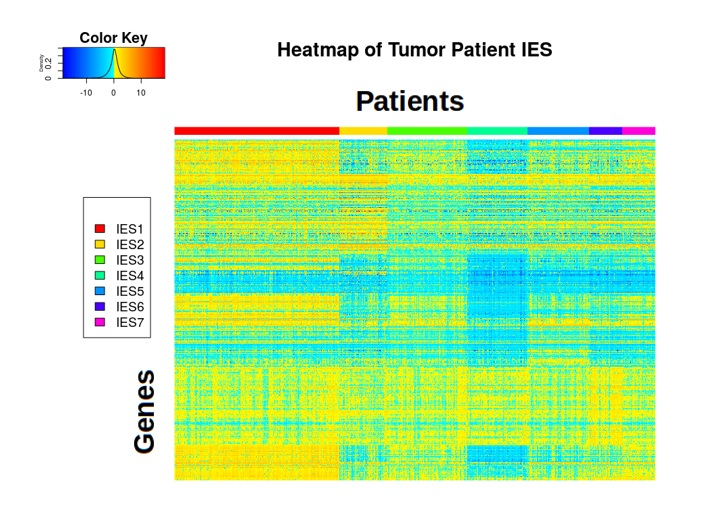
\includegraphics[width=12 cm]{figure4.jpg}
    \caption{Heatmap of study population (breast cancer patients)}
    \label{fig:HM}
  \end{center}
\end{figure}


\subsection*{1.6 Classification Tree with Cross-validation}
After obtaining the $7$ IES, we investigated whether we could identify a small set of genes which could classify the patients into their corresponding IES, In addition, identifying potential biomarker genes will help us understand more about the different mechanisms of immune evasion subtypes, so that we may provide specific guidance on patient selection in combination therapy clinical trials and  on  personalized immunotherapy or combination of immunotherapies.
A classification tree ~\citep{breiman1984classification, atkinson2000introduction} was implemented due to its intuitive output with straight forward clinical interpretations. This analysis was done by the rpart package in \texttt{R}. To validate the robustness of this procedure, a cross validation was also recommended to obtain cross-validated error rates. If the user decide not to implement any cross validation, a reminder message will be printed. Critical part of the source code is given as follows:
\begin{lstlisting}
clftree <- function(X, GroupID, CV = NULL, seed = 1234, fig = TRUE, ...){
	...	
	if (is.null(CV)==1){
    	print("User decide not to do cross validation, although that's highly recommended.")
    	...
  	}
  	set.seed(seed)
  	size_per_fold <- n%/%CV
  	# Use aaa as the randomization scheme
  	# block is the randomized subgroup index. 
  	# Each observation is assigned a value between {1,2,3,...,K}
  	aaa <- rank(runif(n))
  	block <- aaa%%CV + 1
  	Err_clf <- numeric(CV)
  	Mod_clf <- Pred_clf <- list(CV)
  	#This algorithm implements K-fold CV and computes average error rates
  	for (k in 1:CV){
    	Mod_clf[[k]] <- rpart(as.factor(GroupID) ~ ., data = PPI_Tum_RP[block!=k,], 
    	method = "class")
    	Pred_clf[[k]] <- predict(Mod_clf[[k]], newdata = PPI_Tum_RP[block==k,], 
    	type = "class")
    	Err_clf[k] <- sum(Pred_clf[[k]]!=PPI_Tum_RP[block==k,m+1])/sum(block==k)
  }
}
\end{lstlisting}
\begin{itemize}
\item \texttt{X} is the input expression matrix, where we follow the convention that genes are on rows and samples are on columns.
\item \texttt{GroupID} is the vector of cluster labels. For simplicity, we require this input to be a numeric vector of the length of the number of patients. For example, $1$ indicates this patient belongs to cluster 1, etc.
\item \texttt{CV} is the parameter of cross validation. Default $CV=NULL$ means fitting the tree model only once on the complete dataset. A numerical value of $CV$ indicates $CV$-fold cross validation. A reminder message will be printed if the user decide not to implement any cross validation.
\item \texttt{fig} is the parameter of whether to output the fitted classification tree. Default is \texttt{TRUE}, which means a tree figure of resolution $600$ in .png format will be output in the current working directory.
\end{itemize}
The tree is given by Figure~\ref{fig:clftree}. and the $5$-fold average error rate is $29.58\%$.
\begin{lstlisting}
my.mod <- SBic(X = PPI_Tum, propcutoff = 0.05, seed = 1234, outopt = "table", 
	Dataname = "BRCA_RNAseqV2")
my.mod2 <- ttest_general(X = cbind(PPI_Tum, PPI_Nor), 
	classlabel = c(rep("Tumor", 1065), rep("normal", 111)))
## Define patient group ID in the simplest and neatest way
Bic1 <- read.table(file = "BRCA_RNAseqV2_CL1.txt", header = T)
Bic2 <- read.table(file = "BRCA_RNAseqV2_CL2.txt", header = T)
Bic3 <- read.table(file = "BRCA_RNAseqV2_CL3.txt", header = T)
Bic4 <- read.table(file = "BRCA_RNAseqV2_CL4.txt", header = T)
Bic5 <- read.table(file = "BRCA_RNAseqV2_CL5.txt", header = T)
Bic6 <- read.table(file = "BRCA_RNAseqV2_CL6.txt", header = T)
Bic7 <- read.table(file = "BRCA_RNAseqV2_CL7.txt", header = T)
Bic <- list(Bic1, Bic2, Bic3, Bic4, Bic5, Bic6, Bic7)
GROUPID <- rep(0, 1065)
for (i in 1:7){
  GROUPID[which(colnames(PPI_Tum) %in% colnames(Bic[[i]]))]<-i
}
my.mod3 <- clftree(X = PPI_Tum, GroupID = GROUPID, CV = 5, seed = 1234, fig = TRUE)
mean(my.mod3[[2]])
\end{lstlisting}

\begin{figure}[!tpb]
  \begin{center}
    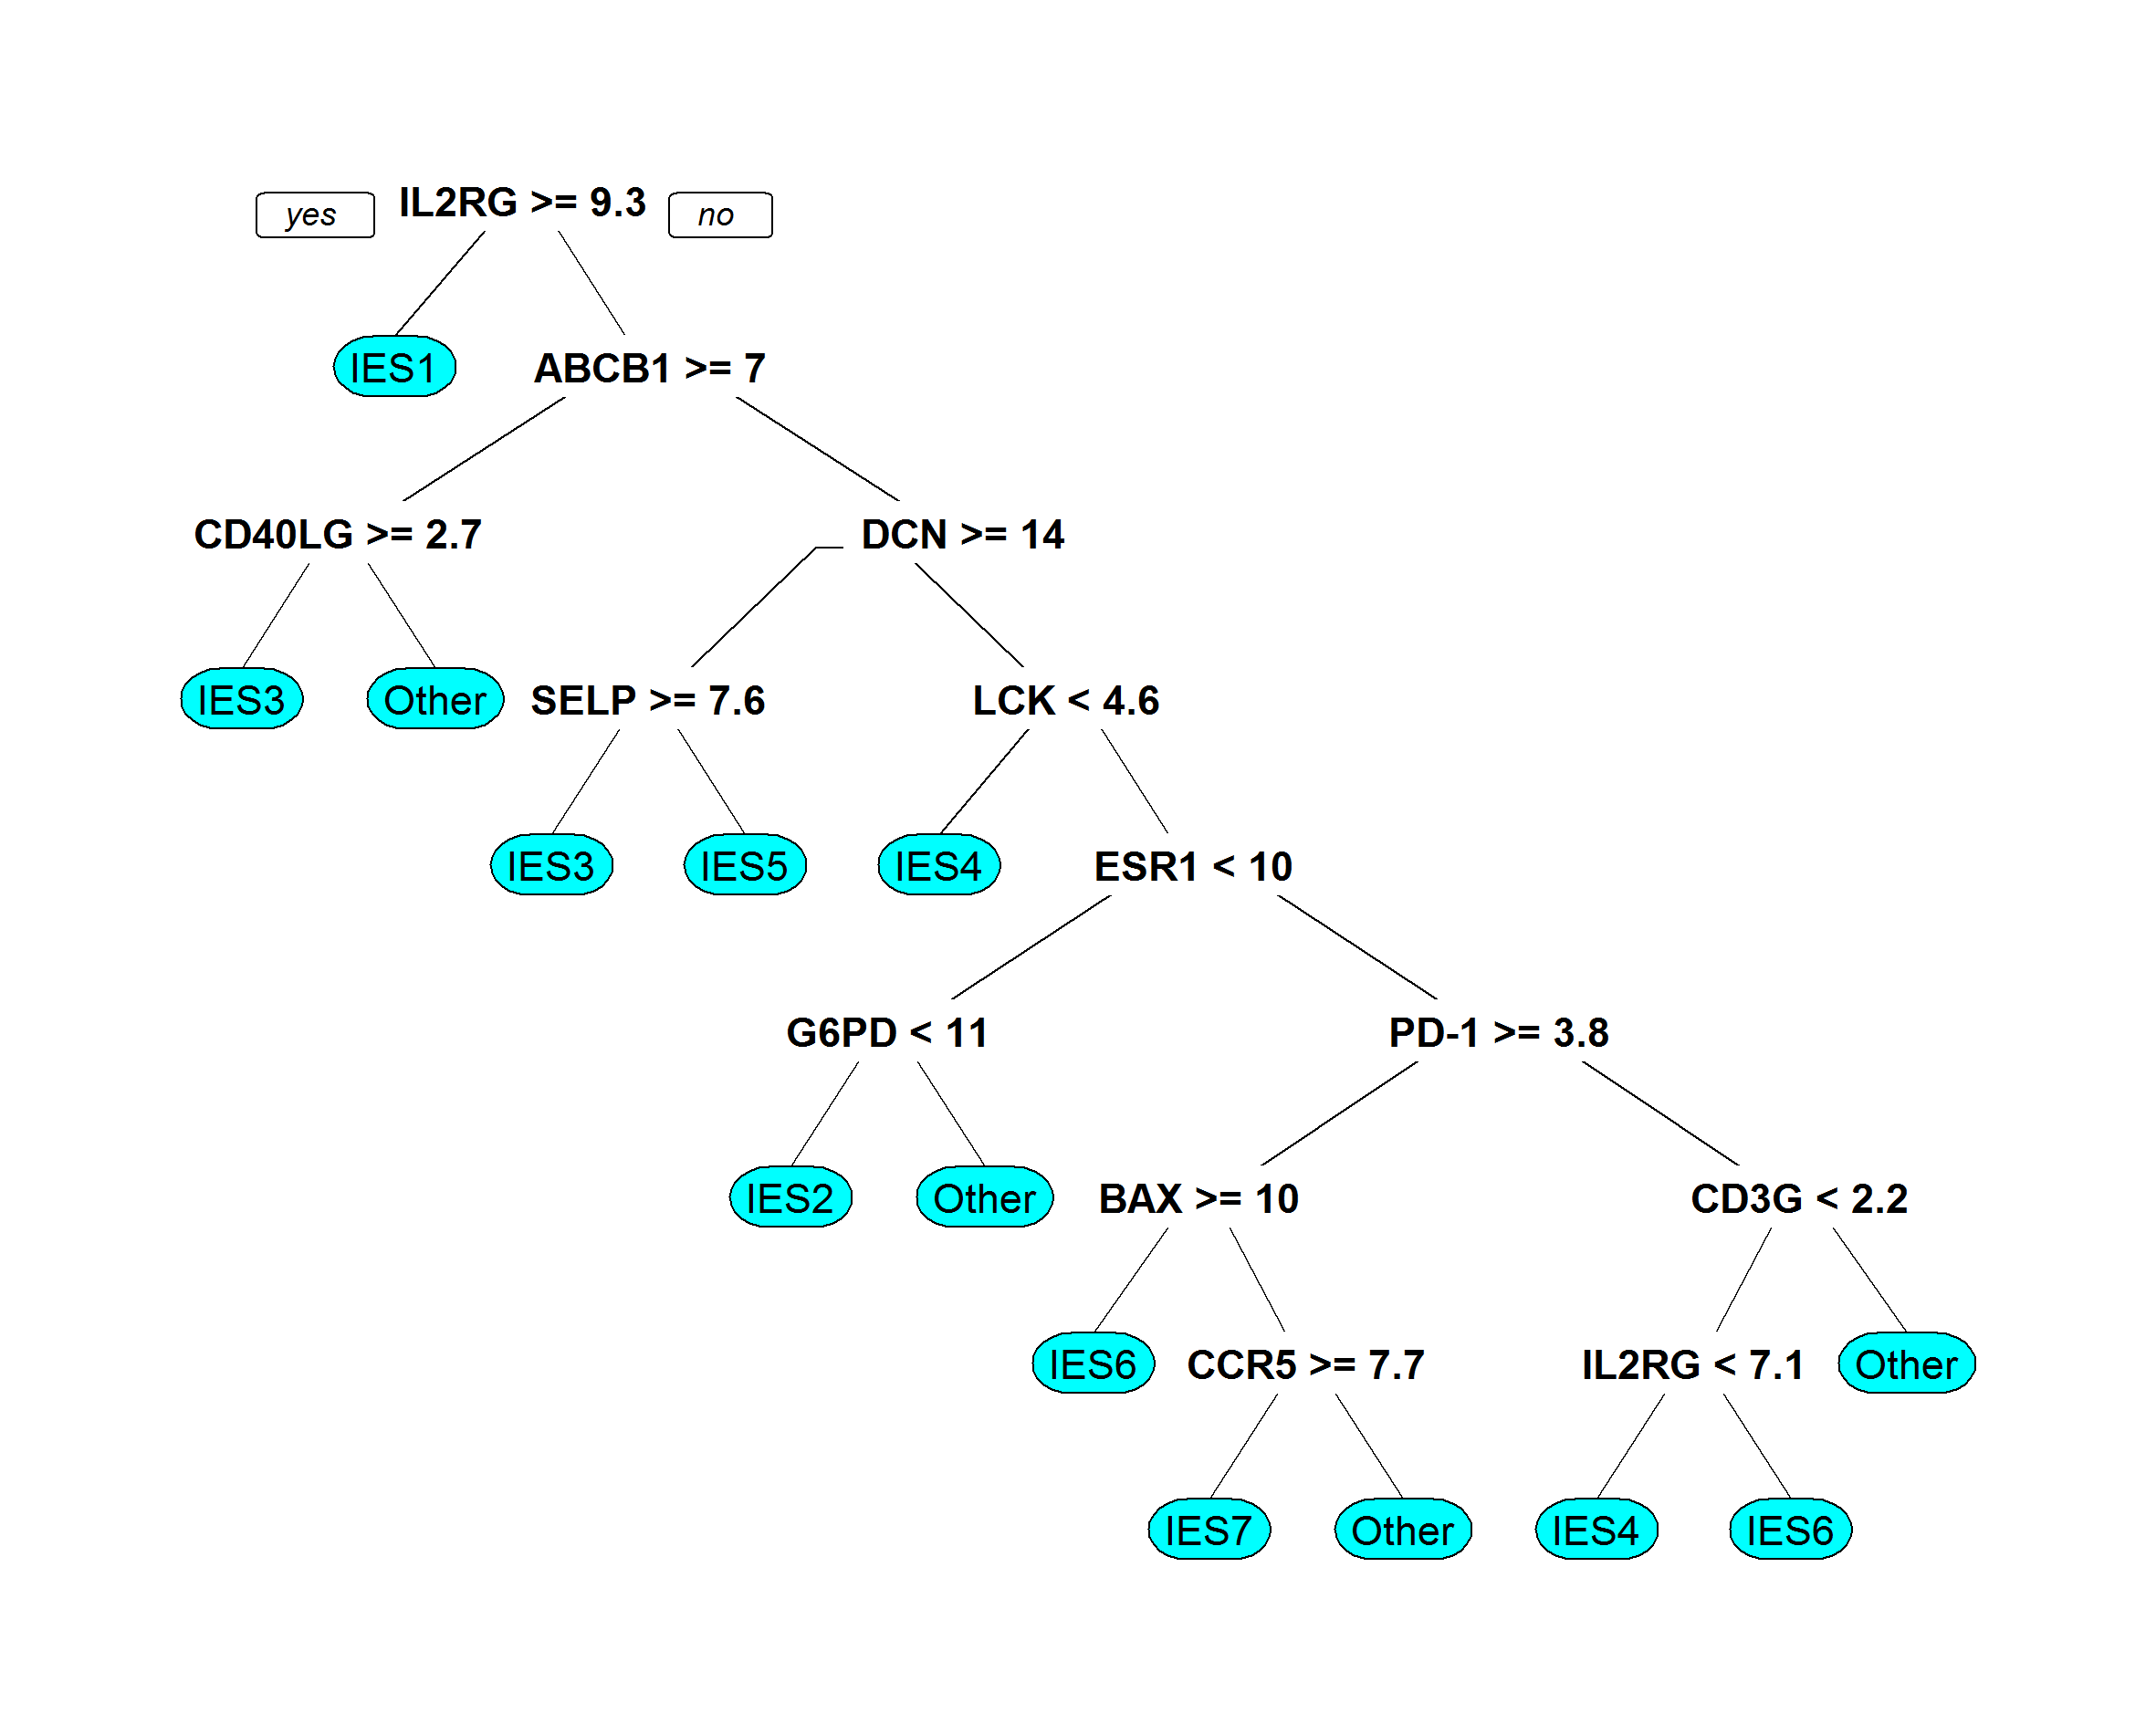
\includegraphics[width=11.5 cm]{figure3.png}
    \caption{Classification tree and important classifier genes to identify IES}
    \label{fig:clftree}
  \end{center}
\end{figure}

\subsection*{1.7 User Prediction of Patient Subtype and Suggested Immunotherapy}
Based on the above classification strategy, we can naturally incorporate a user-friendly function that takes any new (real or simulated) data as input and automatically outputs the patients' IES, related immune evasion mechanism(s), and suggested immunotherapy(ies). With our package, we include an R data frame \texttt{immuno\_table}, that summarizes all the useful information for this part. The function also allows users to develop their own immunotherapy table for different kinds of cancers. Maximizing the degree of flexibility is one of our major concerns.
\begin{verbatim}
user_pred<-function(X,object,mechanism=immuno_table,Dataname="data_sim", ...) {
					...
				}
\end{verbatim}

\begin{itemize}
\item \texttt{X} is the input expression matrix, where we follow the convention that genes are on rows and samples are on columns.
\item \texttt{object} is a model object fitted by any classification function. In this study, we use the classification tree model obtained from the \texttt{clftree} function above.
\item \texttt{mechanism} is the immunotherapy table. Users can develop their own, but we require that to be in a data frame, where the first column is the list of IES, and the second and third columns are the relevant immune evasion mechanisms and immunotherapies respectively.
\item \texttt{Dataname} is an appropriate prefix of the output file name. Its default value is \texttt{data\_simu}, which refers to a simulated dataset. The output table is in .csv format for better readability.
\end{itemize}

\begin{lstlisting}
mean_Tum <- apply(PPI_Tum, 1, mean)
cov_Tum <- cov(t(PPI_Tum))
sim_data <- t(mvrnorm(n = 1000, mean_Tum, cov_Tum))
rownames(sim_data) <- rownames(PPI_Tum)
colnames(sim_data) <- paste("Patient", 1:1000, sep = "")
my.mod4 <- user_pred(X = sim_data, object = my.mod3[[1]], 
	mechanism = immuno_table, Dataname = "data_sim")
my.mod4[1:10,]
   Patient ID   IES      Mechanism                            Suggested Immunotherapies
1    Patient1  IES2             M5                                Ex-vivo modulated DCs
2    Patient2  IES2             M5                                Ex-vivo modulated DCs
3    Patient3  IES3         M2; M4         Ex-vivo modulated DCs; Anti-CTLA4; Anti-DcR3
4    Patient4  IES1 M1; M2; M3; M4           Anti-PD1; Anti-CTLA4; Anti-DcR3; Anti-IFNG
5    Patient5  IES4         M1; M6 Anti-TGF_beta1; Ex-vivo modulated DCs + Chemotherapy
6    Patient6 Other          Other                                                Other
7    Patient7  IES1 M1; M2; M3; M4           Anti-PD1; Anti-CTLA4; Anti-DcR3; Anti-IFNG
8    Patient8  IES1 M1; M2; M3; M4           Anti-PD1; Anti-CTLA4; Anti-DcR3; Anti-IFNG
9    Patient9  IES2             M5                                Ex-vivo modulated DCs
10  Patient10  IES1 M1; M2; M3; M4           Anti-PD1; Anti-CTLA4; Anti-DcR3; Anti-IFNG
\end{lstlisting}

\section*{2 Summary and Concluding Remarks}
Tumors evade immune surveillance using $6$ different mechanisms, which may occur simultaneously in the same tumor (Figure~\ref{fig:immu-mech}). Thus, there are $63$ possible combinations of mechanisms in BRCA. This heterogeneity even at the level of a single cancer hallmark explains the challenge of identifying effective treatments. In the era of immunotherapy and personalized medicine, there is an urgent need for advancing the knowledge of immune evasion in different cancer types and identifying reliable biomarkers that guide both therapy selection and patient inclusion in clinical trials.\\
Using the sequential biclustering method on BRCA RNA-seq data from TCGA, we identified seven IES of BRCA patients that utilize different evasion mechanisms or combination of mechanisms. The mechanisms of evasion were determined based on the expression of immune evasion genes and genes involved in the cancer immunity cycle, and shed light on potential immunotherapies for the corresponding subtypes.\\ 
Of the immunoinhibitory molecules in M1 was IFN-$\gamma$, which was up-regulated in IES 1 and IES 7. IFN-$\gamma$ has contradictory functions with either an anti-tumor or a pro-tumor effect. As an anti-tumor molecule, IFN-γ increases immune cell recruitment and causes a direct inhibition of tumor growth and recognition and elimination by the immune system. Other studies on IFN-$\gamma$ pointed to a pro-tumor role, wherein it was shown to increase Treg development, decrease neutrophil infiltration, aide in tumor proliferation and resistance to apoptosis by CTL and NK cells, and increase PD-L1 expression. In both IES 1 and IES 7, Treg development was increased (CTLA4) in both IES 1 and IES 7, and PD-L1 and anti-apoptotic molecules were up-regulated in IES 1, showing a pro-tumor effect potentially caused by IFN-$\gamma$.\\
Ignorance in IES 4 could have occurred due to cancer cells’ expression of a tumor associated antigen that was recognized by APCs as a ``self" molecule. As suggested in Table 5 of our companion paper, patients in these subtypes can be treated by ex-vivo modulated DCs or CAR-Ts in combination with chemotherapy. Chemotherapy can help antigen recognition by increasing antigen release from dying cancer cells and eliciting an anti-tumor immune response.\\
Going one step further, we also implemented a Fisher exact test ~\citep{fisher1922interpretation, fisher1956mathematics, upton1992fisher} between the patient IES and breast cancer subtype, and found some interesting patterns. The identified immune evasion subtypes 1 and 6 were not significantly associated with any hormone receptor subtype (Luminal A, Luminal B, HER2+, TNBC). However, IES 3, 4, 5, and 7 were significantly associated with Luminal A and IES 2 with TNBC. Due to the higher immune system-tumor interactions involved, TNBC and HER2 were thought to be more immunogenic than Luminal A. However, our results showed that TNBC patients split into two groups: the highly immunogenic IES 1 (TNBC: $51/105=48.57\%$) and the less immunogenic (low leukocyte infiltration) IES 2 (TNBC: $45/105=42.86\%$), indicating that these TNBC patients should be treated differently. Both TNBC and Luminal A associated with different IES may indicate further heterogeneity and complexity of breast cancer.\\

\bibliographystyle{bmc-mathphys} % Style BST file (bmc-mathphys, vancouver, spbasic).
%\bibliographystyle{vancouver}
%\bibliographystyle{spbasic}
\bibliography{SBic}      % Bibliography file (usually '*.bib' )
\end{document} 